\chapter{Results and Discussion}

This chapter reports the results obtained by applying the pipeline to the six-gene panel, with
$100$ sequences requested per gene (and a per-gene override of $200$ for the data-limited
\emph{algD}). It follows the flow of the method: sequence retrieval and
curation, the screening funnel, three-dimensional validation, the diversity and rarefaction
analyses, the effect of the organism-aware parameters, the comparison with the reference panel,
and the curated dataset produced for downstream modelling.

\section{Retrieval and length curation}

Table~\ref{tab:retrieval} shows, for each gene, the number of sequences returned by
\acrshort{ncbi} and the number retained after length clustering. The clustering step removed
partial and oversized records that would otherwise degrade the alignment; its effect is largest
for the genes with the most heterogeneous records. Two genes, \emph{oprL} and \emph{algD},
are intrinsically data-limited in \acrshort{ncbi} (only 24 and 12 sequences survive
respectively), which, as shown below, is reflected in their downstream behaviour.

\begin{table}[H]
\begin{center}
\begin{tabular}{l c c c}
\hline
\textbf{Gene} & \textbf{Retrieved} & \textbf{After clustering} & \textbf{Alignment (cols)} \\
\hline
\emph{nuc}  & 99  & 77 & 517 \\
\emph{rmpM} & 100 & 76 & 1311 \\
\emph{lytA} & 95  & 87 & 2594 \\
\emph{oprL} & 27  & 24 & 770 \\
\emph{algD} & 19  & 12 & 1020 \\
\emph{frdB} & 82  & 82 & 489 \\
\hline
\end{tabular}
\end{center}
\caption{Sequences retrieved and retained per gene, and the resulting alignment width.}
\label{tab:retrieval}
\end{table}

\section{Screening funnel}

Across the six genes, the pipeline generated $8455$ candidate windows and filtered them down to
$2943$ that passed both the thermodynamic screen and the secondary-structure screen
(Table~\ref{tab:funnel}). The melting-temperature and GC filters remove the largest fractions,
as expected, since they encode the core hybridisation requirements; the homodimer filter is
particularly severe for the GC-rich \emph{P.\ aeruginosa} genes (\emph{oprL}, \emph{algD}),
whose sequences are more prone to self-complementarity. The secondary-structure screen removes
only a small additional fraction, confirming that most structurally problematic candidates are
already eliminated by the thermodynamic filters.

\begin{table}[H]
\begin{center}
\begin{tabular}{l c c c c c c}
\hline
\textbf{Gene} & \textbf{Windows} & \textbf{$T_m$} & \textbf{GC} & \textbf{Hairpin} & \textbf{Basic} & \textbf{Seqfold} \\
\hline
\emph{nuc}  & 667  & 326  & 154  & 143  & 143  & 138 \\
\emph{rmpM} & 1867 & 1621 & 1366 & 1251 & 841  & 823 \\
\emph{lytA} & 1833 & 1274 & 966  & 942  & 820  & 771 \\
\emph{oprL} & 1360 & 1273 & 990  & 800  & 349  & 309 \\
\emph{algD} & 1012 & 942  & 763  & 662  & 403  & 389 \\
\emph{frdB} & 1716 & 932  & 752  & 733  & 522  & 513 \\
\hline
\textbf{Total} & \textbf{8455} & \textbf{6368} & \textbf{4991} & \textbf{4531} & \textbf{3078} & \textbf{2943} \\
\hline
\end{tabular}
\end{center}
\caption{Screening funnel: candidate windows surviving each successive filter. ``Basic'' is the
number passing all four thermodynamic criteria; ``Seqfold'' additionally passes the
secondary-structure screen.}
\label{tab:funnel}
\end{table}

\section{Three-dimensional validation}

The five highest-quality candidates per gene ($30$ probes) were validated with Boltz-2. Of
these, $4$ were classified as \textsc{good}, $11$ as \textsc{moderate} and $15$ as \textsc{low}
by the overall confidence. The best candidates, strong \emph{both} in sequence quality and in
3D, are listed in Table~\ref{tab:boltz}; they come from \emph{algD} and \emph{frdB}. The
selected probes are strongly conserved (\acrshort{ppi} up to $1.00$) and essentially free of
self-structure (No-fold above $96$), which coincides with the highest structure-prediction
confidence and \acrshort{plddt} among the $30$ validated probes. The agreement between the
sequence-level signals and the independent 3D prediction provides an internal consistency check
on the ranking.

\begin{table}[H]
\begin{center}
\begin{tabular}{l l c c c c}
\hline
\textbf{Probe} & \textbf{Gene} & \textbf{\acrshort{ppi}} & \textbf{No-fold} & \textbf{Confidence} & \textbf{\acrshort{plddt}} \\
\hline
p5972 & \emph{algD} & 0.93 & 98.4 & 0.731 & 0.901 \\
p7716 & \emph{frdB} & 0.99 & 99.6 & 0.723 & 0.822 \\
p5938 & \emph{algD} & 0.90 & 96.2 & 0.721 & 0.887 \\
p8448 & \emph{frdB} & 1.00 & 98.2 & 0.716 & 0.845 \\
\hline
\end{tabular}
\end{center}
\caption{Top probe candidates, strong in both sequence quality and 3D confidence.}
\label{tab:boltz}
\end{table}

\section{Genetic diversity of the targets}

The alignment-free diversity analysis (Table~\ref{tab:diversity}) explains much of the
behaviour observed above. \emph{lytA} is by far the most diverse gene (mean cosine distance
$0.187$ and $93\%$ unique sequences), consistent with its known allelic diversity in
\emph{S.\ pneumoniae} \citep{obregon2002}; this justifies the relaxed conservation threshold
applied to it. At the opposite extreme, \emph{frdB} is the most conserved and most redundant
gene (mean cosine distance $0.025$ and only $35\%$ unique sequences, i.e.\ many exact
duplicates in \acrshort{ncbi}), which is why it yields probes of very high conservation.
\emph{algD} has $100\%$ unique sequences but very few of them, which accounts for its
instability at low sampling and motivates the automatic length-clustering and the per-gene
allowance of more sequences. The cosine and Jaccard distances are complementary --- the former
weighs $4$-mer frequencies, the latter only their presence or absence --- and they concur in
identifying \emph{frdB} as the most conserved and redundant gene, giving an alignment-independent
reading of diversity.

\begin{table}[H]
\begin{center}
\begin{tabular}{l c c c c c}
\hline
\textbf{Gene} & \textbf{$n$} & \textbf{Cosine (mean)} & \textbf{Cosine (max)} & \textbf{Jaccard (mean)} & \textbf{Unique (\%)} \\
\hline
\emph{nuc}  & 77 & 0.059 & 0.425 & 0.163 & 61.0 \\
\emph{rmpM} & 76 & 0.079 & 0.247 & 0.069 & 50.0 \\
\emph{lytA} & 87 & \textbf{0.187} & 0.440 & 0.125 & 93.1 \\
\emph{oprL} & 24 & 0.050 & 0.358 & 0.096 & 91.7 \\
\emph{algD} & 12 & 0.097 & 0.332 & 0.117 & \textbf{100.0} \\
\emph{frdB} & 82 & \textbf{0.025} & 0.052 & 0.061 & \textbf{35.4} \\
\hline
\end{tabular}
\end{center}
\caption{Alignment-free $k$-mer diversity per gene. Bold marks the most diverse (\emph{lytA})
and the most conserved/redundant (\emph{frdB}) genes.}
\label{tab:diversity}
\end{table}

\begin{figure}[H]
\begin{center}
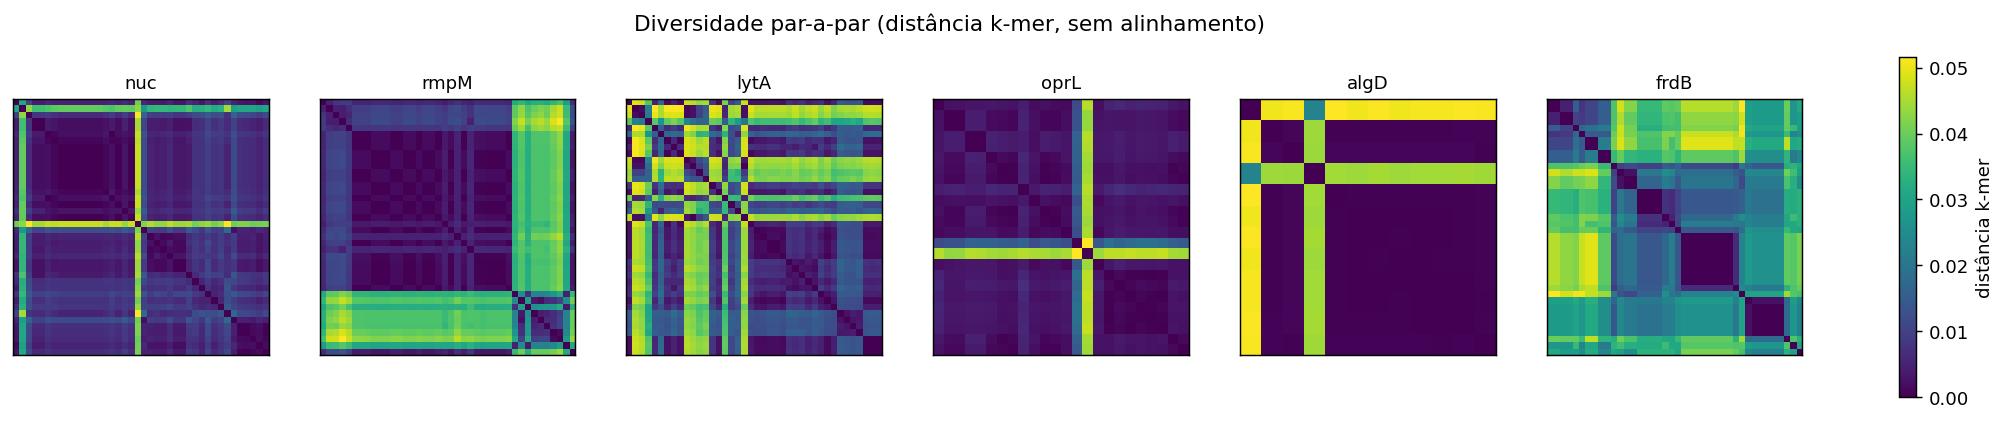
\includegraphics[width=\textwidth]{images/diversity_heatmaps.png}
\end{center}
\caption{Pairwise $4$-mer distance heatmaps per gene (alignment-free). Each cell is the $4$-mer
distance between two retrieved sequences of the gene.}
\label{fig:diversity}
\end{figure}

\section{Choice of sampling depth}

The rarefaction analysis showed that both the $4$-mer diversity and the $4$-mer richness
saturate at around $N \approx 50$ sequences for the most demanding gene (\emph{nuc}), and much
earlier for the others. Requesting up to $100$ sequences per gene therefore captures essentially
all of the available diversity with a comfortable margin, while additional sequences add little
new information. The true limiting factor is not this cap but the small number of records
available in \acrshort{ncbi} for the data-limited genes.

\begin{figure}[H]
\begin{center}
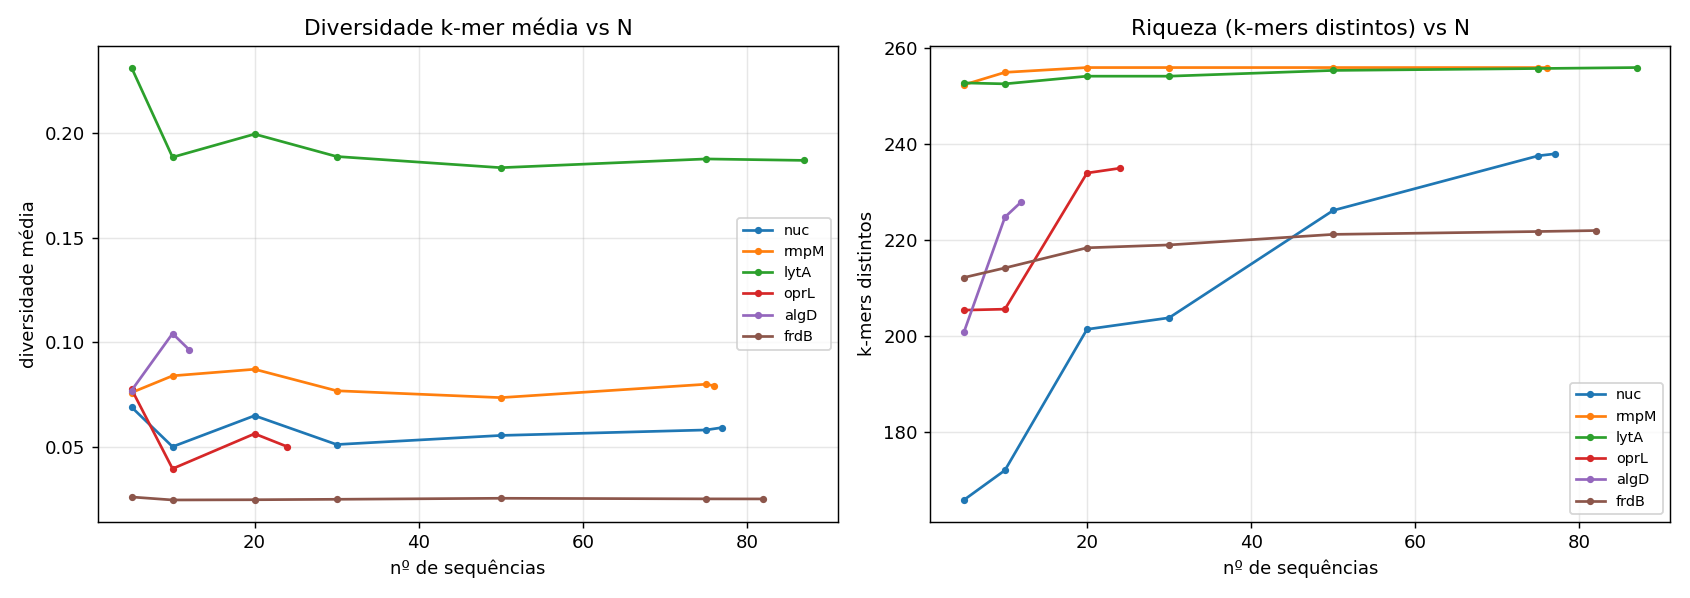
\includegraphics[width=\textwidth]{images/rarefaction.png}
\end{center}
\caption{Rarefaction of the mean $4$-mer diversity (left) and of the richness, i.e.\ the number
of distinct $4$-mers (right), per gene, as a function of the number of subsampled sequences.}
\label{fig:rarefaction}
\end{figure}

\section{Effect of the organism-aware parameters}

The value of resolving thresholds per organism type and species is clearest when scoring the
reference panel, which spans bacteria, viruses, a fungus, a protozoan and a human control. When
the $74$ reference probes were scored with a single global (bacterial) criterion, $29$ passed
the basic screen; when instead each was scored by the criteria of its own species and type,
$39$ passed. The additional probes are precisely those whose genome composition differs from
the balanced bacterial case --- for example the AT-rich \emph{Plasmodium} probe, which the
global GC window would reject but which is appropriate under the protozoan profile. This
confirms that organism-aware thresholds avoid unfair rejections without loosening the criteria
for the balanced targets.

\section{Comparison with the reference panel}

Scored with identical metrics, the designed probes and the reference panel can be compared
directly. Among the probes that pass the basic screen, the designed probes have a higher mean
melting temperature ($59.3$ versus $56.9\,^{\circ}$C) and a very similar mean GC content ($0.52$
versus $0.53$), while the reference probes have a marginally higher mean No-fold score ($86.0$
versus $82.9$). Because both sets carry a source label and share every column, they can also be
submitted together to Boltz-2, enabling a like-for-like comparison in three dimensions as well as
in sequence space.

\section{Curated dataset for downstream modelling}

Finally, the same quality ranking was used to export a larger curated dataset: the top $25$
probes per gene ($150$ probes in total), each with its sequence-level features (\acrshort{tm},
GC, conservation, No-fold and folding energies). This dataset extends the small set validated
in 3D and provides biophysically annotated candidates for the data-driven modelling of probe
quality that is a natural continuation of this work.
